\documentclass[12pt]{article}

\usepackage[utf8x]{inputenc} % Включаем поддержку UTF8  
\usepackage[russian]{babel}  % Включаем пакет для поддержки русского языка  
\usepackage{hyperref}        % Для гиперссылок

% Математика
\usepackage{amsmath}         % В т.ч. для матриц
\usepackage{amssymb}

% Прога
\usepackage{etoolbox}
\usepackage{listings}

% Цвета
\usepackage{xcolor}

% Картинки
\usepackage{graphicx}
\graphicspath{ {./images/} }

\newtheorem{property}{Свойство}
\newtheorem{consequence}{Следствие}[property]

\newcommand{\qedsymbol}{\rule{2mm}{2mm}}

\begin{document}

\thispagestyle{empty}
\begin{center}
\textbf{ПРАВИТЕЛЬСТВО РОССИЙСКОЙ ФЕДЕРАЦИИ}

\vspace{5ex}
	
\textbf{Федеральное государственное автономное образовательное учреждение \\ высшего образования \\ <<Национальный исследовательский университет \\ <<Высшая школа экономики>>}
\end{center}
\vspace{5ex}

\begin{center}
    Московский институт электроники и математики им. А.Н. Тихонова  
    
    \vspace{5ex}
    
    Департамент прикладной математики
    
    \vspace{10ex}
    \textbf{Отчёт \\ по лабораторной работе №5 \\ по курсу <<Алгоритмизация и программирование>>}
	\vspace{7ex}

\end{center}

\begin{center} 
\begin{tabular}{| p{0.3\linewidth}| p{0.3\linewidth}| p{0.3\linewidth}|}
 \hline	
ФИО студента & Номер группы & Дата \\  \hline
 & & \\  
Вязов Глеб \newline Дмитриевич & БПМ-231 & 18.11.2023\\  
 & & \\  \hline		
\end{tabular}
\end{center}

\begin{center}
	\vspace{3ex}
	
	\vfill
   
   \normalsize
    
	\textbf{Москва, 2023}
\end{center}

\newpage

%---------------------------------------------------------------------------------

\section*{Задание (вариант №7)}
Дана целочисленная матрица размера mxn, где $2 \leq m, n \leq 10$.
Программа должна быть разбита на несколько функций и обязательно содержать:
\begin{enumerate}
\item функцию формирования исходного массива;
\item функцию вывода исходного массива;
\item одну или более функций, реализующих вычислительную часть алгоритма.
\end{enumerate}
Все функции должны содержать список параметров, причём адрес массива должен передаваться как параметр функции. Функция
main должна содержать только операторы вызова функций.
Использовать статический массив. Дополнительных массивов не использовать!

\newpage

%---------------------------------------------------------------------------------

\section*{Решение}\addcontentsline{toc}{section}{Решение}

\lstset{ %
texcl=true,%
language=C,                 % выбор языка для подсветки
basicstyle=\small\sffamily, % размер и начертание шрифта для подсветки кода
numbers=left,               % где поставить нумерацию строк (слева\справа)
numberstyle=\tiny,           % размер шрифта для номеров строк
stepnumber=1,                   % размер шага между двумя номерами строк
numbersep=5pt,                % как далеко отстоят номера строк от подсвечиваемого кода
backgroundcolor=\color{white}, % цвет фона подсветки - используем \usepackage{color}
showspaces=false,            % показывать или нет пробелы специальными отступами
showstringspaces=false,      % показывать или нет пробелы в строках
showtabs=false,             % показывать или нет табуляцию в строках
frame=single,              % рисовать рамку вокруг кода
tabsize=3,                 % размер табуляции по умолчанию равен 2 пробелам
captionpos=t,              % позиция заголовка вверху [t] или внизу [b] 
breaklines=true,           % автоматически переносить строки (да\нет)
breakatwhitespace=false, % переносить строки только если есть пробел
escapeinside={\%*}{*)},   % если нужно добавить комментарии в коде
inputencoding=utf8x,
extendedchars=\true
}

\begin{lstlisting}[label=string_code1,caption=C]
#include <stdio.h>

int const NMAX = 100;

// Создаем массив
void create_array(int array[][NMAX], int *pm, int *pn) {
    printf("Введите количество строк массива: ");
    scanf("%d", pm);
    printf("Введите количество столбцов массива: ");
    scanf("%d", pn);

    for (int i=0; i<*pm; i++) {
        for (int j=0; j<*pn; j++) {
            scanf("%d", &array[i][j]);
        }
    }
}

// Вывод массива
void print_array(int array[][NMAX], int m, int n) {
    for (int i=0; i<m; i++) {
        for (int j=0; j<n; j++) {
            printf("%d\t", array[i][j]);
        }
        printf("\n");
    }
}

// Функция возвращает максимальное количество четных чисел в строке
int max_even_in_line(int array[][NMAX], int m, int n) {
    int max_even = 0;
    for (int i=0; i<m; i++) {
        int current_max_even = 0;
        for (int j=0; j<n; j++) {
            if (array[i][j] % 2 == 0) {
                current_max_even++;
            }
        }

        // Если в этой строке четных элементов больше, то запоминаем
        if (current_max_even > max_even) {
            max_even = current_max_even;
        }
    }
    return max_even;
}

// Функция возвращает сумму элементов, та тех строках, на которых кол-во
// четных элементов максимально
int sum_max_even(int array[][NMAX], int m, int n) {
    int sum = 0;
    int max_even = max_even_in_line(array, m, n);

    for (int i=0; i<m; i++) {
        int current_max_even = 0;
        int current_sum = 0;
        
        for (int j=0; j<n; j++) {
            current_sum += array[i][j];
            if (array[i][j] % 2 == 0) {
                current_max_even++;
            }
        }

        // Если в этой строке количество четных элементов -- максимально
        // То добавляем сумму элементов на этой строке
        if (current_max_even == max_even) {
            sum += current_sum;
        }
    }

    return sum;
}

int main() {
    // Меняем кодировку на UTF-8, чтобы можно было писать на русском
    system("chcp 65001");
    // Ввод переменных. Дружественный интерфейс
    printf("Выполнил задание: Вязов Глеб. Группа: БПМ231\n");

    int array[NMAX][NMAX];
    unsigned int m, n;

    create_array(array, &m, &n);
    printf("Вы создали массив:\n");
    print_array(array, m, n);
    printf("Сумма элементов тех строк, которые содержат наибольшее число чётных элементов: %d",
           sum_max_even(array, m, n));

    return 0;
}
\end{lstlisting} 

\newpage

%---------------------------------------------------------------------------------

\section*{Тестирование}

\begin{enumerate}

\item \textbf{Тест №1.} 

\textit{Ввод:} 
$m=3, n=3$
Элементы матрицы: 2, 3, 4, 5, 6, 7, 8, 9, 10

\textit{Вывод:} 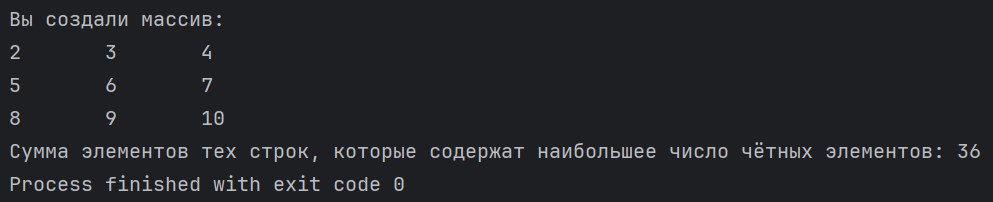
\includegraphics[width=0.9\textwidth]{img1}



\item \textbf{Тест №2.}

\textit{Ввод:}
$m=3, n=2$
Элементы матрицы: 1, 2, 3, 4, 5, 6

\textit{Вывод:} 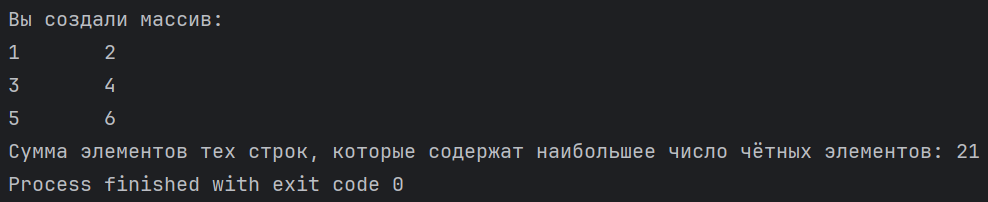
\includegraphics[width=0.9\textwidth]{img2}



\item \textbf{Тест №3.}

\textit{Ввод:}
$m=2, n=3$
Элементы матрицы: 1, 2, 3, 4, 5, 6

\textit{Вывод:} 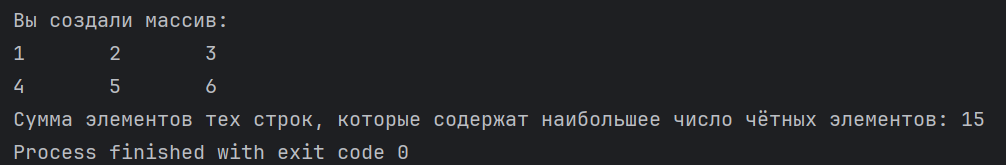
\includegraphics[width=0.9\textwidth]{img3}


\end{enumerate}


\end{document}
